\documentclass[twocolumn]{report}	
\title{\textsc{\Huge Polar Codes} \\ \textsc{Primary Concepts and
Practical Decoding Algorithms}}

\author{\textbf{Member 1: Himanshu Sharma [1610110149]} \\ \textbf{Member 2: Dhruv Mehra [1610110119]} \\ \textbf{Member 3: Ram Charan [1610110093]} \\\\ {\it Under the guidance of Prof. Vijay K. Chakka} \\\\\\ \LARGE{Dept. of Electrical Engineering} \\\\\\ \textsc{(Midterm Evaluation Report)} \\\\\\\LARGE{Shiv Nadar University} \\ NH91, Tehsil Dadri, Greater Noida, Uttar Pradesh 201314}

\date{}
\renewcommand{\thesection}{\arabic{section}}
\usepackage[margin=1.1in]{geometry}
\usepackage{graphicx}
\usepackage{float}
\usepackage{amsmath}

\begin{document}
\maketitle

\section{Introduction}
Polar Codes are an emerging class of error correcting codes. Error correcting codes are used to detect the errors  that arise from the noisy channel through which the data is transmitted and then appropriately removing its effect. Many such codes exist already in the field of \textit{Information Theory}. Hamming codes are one of the popular classes of error correcting codes. Polar codes are new and emerging class of these types of codes.

\par There is something called channel coding which basically means that we code a stream of data at the transmitter end by some set of mathematical operations and then at the  receiver side the reverse operations are done to get back the orignal data stream. Together these operations are called \textit{encoding} and \textit{decoding} respectively. The basic requirement when designing a new error correcting code is to make it less complex, because if the code complexity is increased, then the power consumption, memory consumption, computation power, etc increase at a fast rate. Polar codes have a complexity of $\mathcal{O}(n \log n)$. 

\par There are two types of channel coding schemes, these are, \textit{block coding} and \textit{convolutional codes}.  Block codes work on a block of data/bits with fixed size and apply the manipulation to this block at the transmitter and receiver. Reed-Solomon codes, commonly used on the hard disks of computers, are one example of this type of code. Convolutional codes, on the other hand, work on streams of data with more arbitrary numbers of data/bits. These codes apply a sliding window method that provides a substantial decoding benefit. Simple Viterbi codes are an example of this type of code.

\par Polar codes come under the category of block codes. Their approach is remarkably different. In many ways, polar codes represent techniques similar to that performed in the \textit{fast Fourier transform}. There are two processes involved in this technique, first, \textit{channel combining} and \textit{channel splitting}. Channel combining is similar to what happens in OFDM. In channel combining, the encoder, combines group of bits and assigns that group to a particular channel. The channel splitting that follows performs an implicit transformation operation (analogous to frequency domain to time domain as performed by an IFFT operation), translating these bit/symbol combinations into decoder-ready, time domain vectors.  The real magic in polar codes lies in the clever bit manipulations and mappings to the channels at the encoder. The original technique, in combination with channel splitting, and successive-cancellation decoding, is shown to essentially convert a block of bits, and their associated channels between the encoder and decoder, into a polarized bit stream at the receiver. That is a received bit and its associated channel ends up being either a “good channel” or “bad channel” pole/category. It has been mathematically proven that as the size of the bit block increases, the received bit stream polarizes in a way that the number of “good channels” approaches Shannon capacity. This phenomenon is what gives polar codes their name and makes them the first and only explicitly proven capacity-achieving practical channel codes ever conceived.

\subsection{Shannon's Channel Coding Theorem}
The Shannon's channel coding theorem states that any channel has certain capacity upto which bits can be transmitted through it without being affected too much by noise. The maximum capacity is called \textit{Shannon's limit}. The capacity $C$ in general, is given by 
\begin{equation}
C = I(X;Y) = \log_{2}\frac{P(y_{j}|x_{i})}{P(y_{j})}
\end{equation}
where, $X$ and $Y$ denotes two random variables which acquire a value $x_{i}$ and $y_{j}$ at random and $P$ denotes probability. Now, the entropy of the channel is given by 
\begin{equation}
H = \sum_{i=1}^{m}P_{i}\log_{2}\Bigg(\frac{1}{P_{i}}\Bigg)
\end{equation}
Note that $m$ denotes the number of symbols in a transmission. If an event is sure, then its entropy is 0, becuase for a sure event $P = 1$ and thus making $H=0$. The maximum entropy occurs when all the symbols are equally probable, i.e., $P_{i} = \frac{1}{m}$.
\begin{center}
$\displaystyle H = \sum_{i=1}^{m}\frac{1}{m}\log_{2}(m) = \log_{2}(m) = H_{max}$
\end{center}

\subsection{Asymptotic Equipartition Property}
This property states that in a long turn, random sequences which are \textit{iid} will tend to have a uniform distribution. Consider a biased coin having \textit{head} probability of 0.7 and \textit{tail} probability of 0.3. In a trial of 10 tosses, it is likely that out of 10, only 5 coins come out to be head. But if the trials are 10,000, then it is obvious that heads will occur mostly 7000 times. Mathematically,
\begin{center}
$ \displaystyle \lim_{N \rightarrow \infty}\frac{n(H)}{N} =p $
\end{center}
where $p$ is the probability of getting heads $H$ and $N$ is the total number of trials. To utilize the full channel capacity, many error correcting codes have been used like LDPC and turbo codes.

\subsection{Channel Polarization}
At first some independent channels are separated out by the order of their reliability. Separating channels based on their reliability is important because it determines which channel would be suitable for transmitting the information. Applying this algorithm recursively, which is used to separate them out on the basis of their reliability, we find that at the final stage all the ``good" and ``bad" channels are separated out. This process of separating out the channels as useless and useful is called \textit{channel polarization}.

\subsection{The $Q$ Function}
The $Q$ function is something that will be widely used in this paper. $Q$ function is defined as follows
\begin{equation}
\displaystyle Q(x) = \int_{x}^{\infty}\frac{1}{\sqrt{2\pi}}e^{-\frac{z^{2}}{2}}dz
\end{equation}
The graph of the Q function is shown below.
\begin{figure}[H]
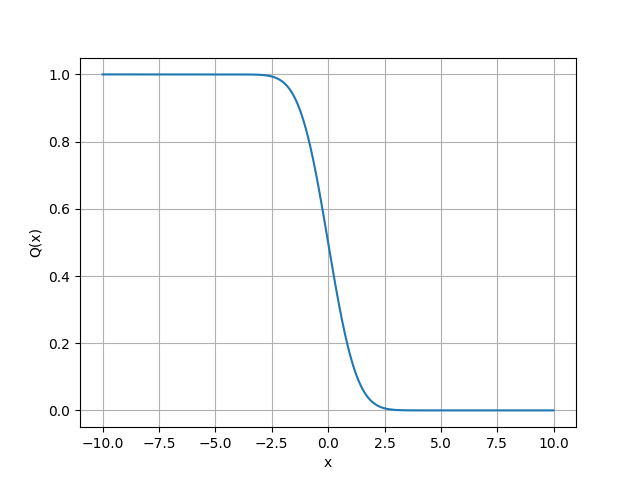
\includegraphics[width=0.55\textwidth, height=0.4\textwidth]{qfunc.png}
\caption{The $Q$ Function}
\end{figure}
The $Q$ function is also expressible as shown below.
\begin{equation}
Q(x) = \frac{1}{2}\textrm{erfc}{\frac{x}{\sqrt{2}}}
\end{equation}
From equation (2), it is clear that for a random variable $X$ with mean $\mu$ and standard deviation $\sigma$ following a normal distribution, when standardized, will form a yet another normal distribution $Z$ such that $\displaystyle Z = \frac{X-\mu}{\sigma}$. $Q$ function can also be defined now in terms of probability of the random variable $Z$.
\begin{equation}
Q(x) = P(X>x)
\end{equation}
An important property of $Q$ function is $Q(x) = 1 - Q(-x)$.

\subsection{Bit Error Rate}
Whenever we transmit a signal over some communication channel, the original signal is modified by the noise. The bit error rate or BER for short, is the probability that a received symbol $\hat{s}$ is not equal to the original transmitted symbol $s$. Mathematically saying, $BER = P(s \neq \hat{s})$. Consider the case of BPSK. If the logic 1 is denoted by $\sqrt{E_{b}}$ and logic 0 is denoted by $-\sqrt{E_{b}}$ where $E_{b}$ is the energy per bit of the symbol, then BER is given as 
\begin{equation}
\displaystyle BER = Q\Bigg(\sqrt{\frac{2RE_{b}}{N_{0}}}\Bigg)
\end{equation}
where, $R$ is the rate of transmission. For uncoded case, $R=1$.
If we plot $\log(BER)$ vs $E_{b}/N_{o}$ ratio (in dB), then the following curve is generated,
\begin{figure}[H]

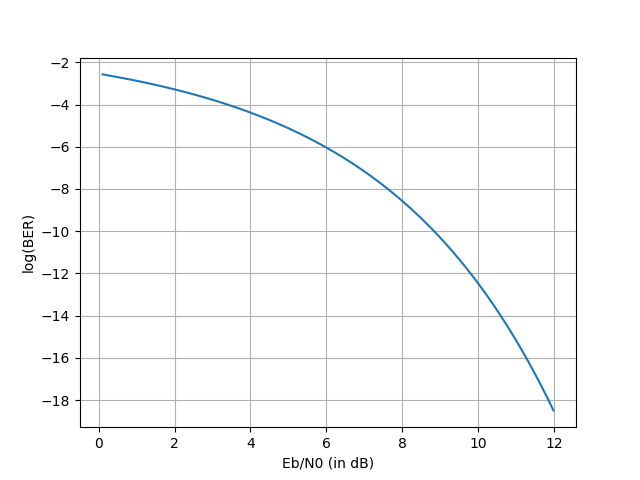
\includegraphics[width=0.55\textwidth, height=0.3\textheight]{bervsebno.png} 
\caption{$\log(BER)$ vs. $E_{b}/N_{o}$ (in dB)}
\end{figure}
Below, a graph has been shown just to compare the theoretical and simulated BER results.
\begin{figure}[H]
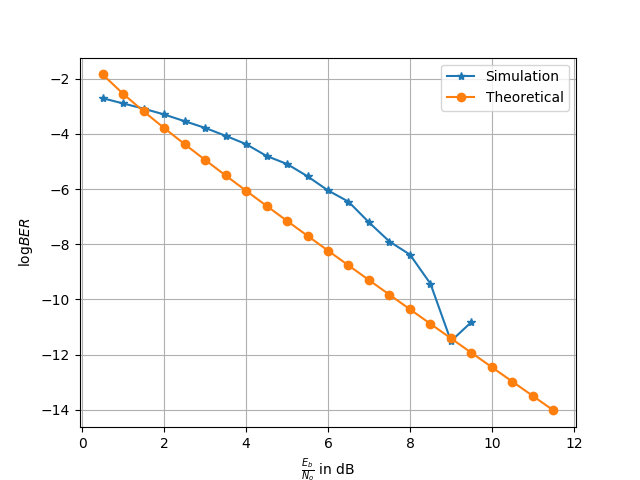
\includegraphics[width=0.5\textwidth, height=0.3\textheight]{thvspr_uncoded.png}
\end{figure}
Later on, in this paper, it will be shown that the theoretical and the simulated BER are same.


\subsection{$n=3$ Repetition Codes}
Using codes is beneficial in transmission because they reduce the bandwidth consumption. Consider the block diagram given below.
\begin{figure}[H]
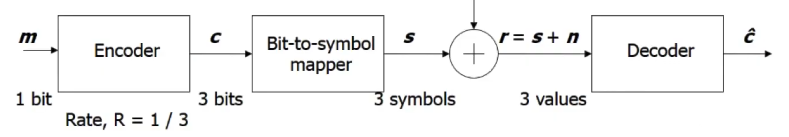
\includegraphics[width=0.5\textwidth, height=0.07\textheight]{repitioncode.png}
\end{figure}
This block diagram corresponds to the binary transmission only, i.e., the input to the encoder is either 1 or 0. The encoder maps 1 to 111 and 0 to 000 and thus changing the rate to $R=1/3$. Since the bits are repeated, it is called the repetition code. The bits to symbol mapper maps these symbols to $[1,1,1]$ for 000 and $[-1, -1, -1]$ for 111. The signals are then transmitted in an AWGN medium. The BER, in general for rate $R$ is given by $\displaystyle BER = Q\Bigg(\sqrt{\frac{1}{R\sigma^{2}}}\Bigg)$. Hence, here, in this case, BER is $\displaystyle Q\Bigg(\sqrt{\frac{3}{\sigma^{2}}}\Bigg)$.
\par Generally, we always try to make $E_{b}/N_{o}$ ratio to be same in both coded and uncoded case and hence we can do the following;
\begin{center}
$\displaystyle \frac{1}{2R\sigma_{coded}^{2}} = \frac{1}{2\sigma_{uncoded}^{2}}$
\end{center}
Since, $R<1$, we get, $\sigma_{coded} > \sigma_{uncoded}$. That is, noise is more probable in coded case. It is also evident from the curves shown below. 
\begin{figure}[H]
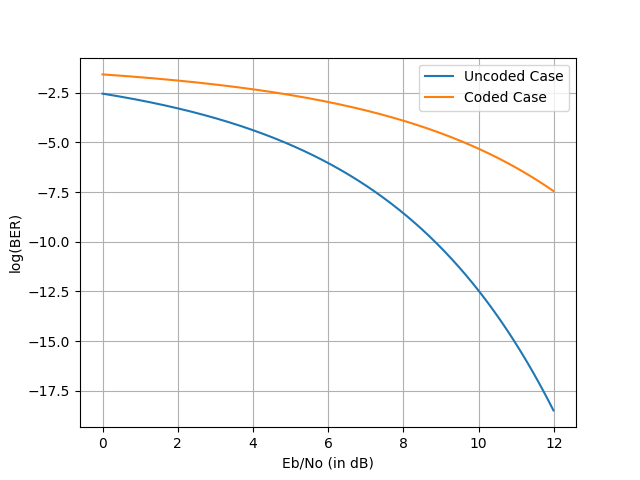
\includegraphics[width=0.5\textwidth, height=0.3\textheight]{codedvsuncoded.png}
\caption{$\log{BER}$ vs $E_{b}/N_{o}$ ratio for Uncoded and Coded case}
\end{figure}
It is evident from the curves that for the same $E_{b}/N_{o}$ ratio, the coded case gives higer bit error rate. This is the disadvantage of the coding schemes. They introduce more BER but reduce bandwidth consumption.
\par Now after passing through AWGN, if the vector $[r_{1}, r_{2}, r_{3}]$ is received, then the symbol $\hat{c}$ can be found out by comparing the distance from the ideal symbols;
\begin{center}
$|r - [1,1,1]| < |r-[-1,-1,-1]| \implies \hat{c} = 000$ 
\end{center}
On further simplification, it states that if
\begin{center}
$r_{1}+r_{2}+r_{3} > 0 \implies \hat{c} = 000$
\end{center}
\subsection{$(7, 4)$ Hamming Code}
A $(7, 4)$ hamming code is something similar to repetition code but not exactly like it. In this type of coding, 4 bits of symbol is coded as a 7 bits symbol. The extra 3 bits that are added were decided after extensive research. After the 7 bits are formed, the symbols are transmitted over AWGN channel and the vector $r$ is received. At the side of the receiver, either a \textit{hard decision} or a \textit{soft decision} is made. 
\subsubsection{Hard Decision}
In this form of decision making process, if $r_{i} > 0 \implies b_{i} = 0$ and vice versa. After the $b$ vector is formed, the hamming distance is calculated from the original mapping. The original mapping which has the least hamming distance, that mapping is decided as the output.
\subsubsection{Soft Decision or ML Decision}
In this form of decision making process, the norm is taken, just as we did in the repetition code case, and then the final symbol is decided.

\subsection{Linear Block Codes}
Consider a message stream of $k$ bits and an encoder which codes them into $n$ bits. We define a generator matrix $G$ such that it generates a codeword matrix $C$ as follows;
\begin{equation}
C = MG
\end{equation}
where, $G = [IP]$, $P$ is the parity matrix and $M$ is the matrix for message bits. Also, the inverse relation of this equations stands as a parity check.
\begin{equation}
[P^{T}I]C^{T} = [0]
\end{equation}
Note that all the additions are modulo 2.

\section{Polar Transform}
Before we discuss the polar codes, its important that we know what is a polar transform. Its something \textit{similar} to FFT and IFFT. We define a transform matrix or generator matrix $G_{2}$ for it, where,
\[
G_{2}=
\begin{bmatrix}
1 & 0 \\
1 & 1
\end{bmatrix}
\]
If we consider a message vector \[ U = \begin{bmatrix} u_{1} \\ u_{2} \end{bmatrix} \], then the polar transform of this message vector will be $U^{T}G$.
\[
U^{T}G_{2} = 
\begin{bmatrix}
u_{1} &
u_{2}
\end{bmatrix}
\begin{bmatrix}
1 & 0 \\
1 & 1
\end{bmatrix}
= 
\begin{bmatrix}
u_{1} + u_{2} &
u_{2}
\end{bmatrix}
\]
This was only the case until we considered two message symbols. If we have $N$, in general, message symbols, then the $G$ matrix is generated by the \textit{Kornecker product}.
\begin{equation}
G_{k} = G_{2} \otimes G_{k/2}
\end{equation}
More appropriately,
\[
G_{k} = 
\begin{bmatrix}
1 & 0 \\
1 & 1
\end{bmatrix}
\otimes
G_{k/2}
= 
\begin{bmatrix}
G_{k/2} & 0 \\
G_{k/2} & G_{k/2}
\end{bmatrix}
\]
\section{Channel Polarization}
The concept of channel polarization is simple. The information bits are transformed into polar domain by the application of suitable polar transform matrix. The point of applying is polar transform is simple; if we don't apply a polar transform on the bits, the bits goes simply like they would have gone in the case of simple BPSK. Applying the polar transform on these bits, changes the channel in such a way that now each bit has its own bit channel.
\begin{figure}[H]
\centering 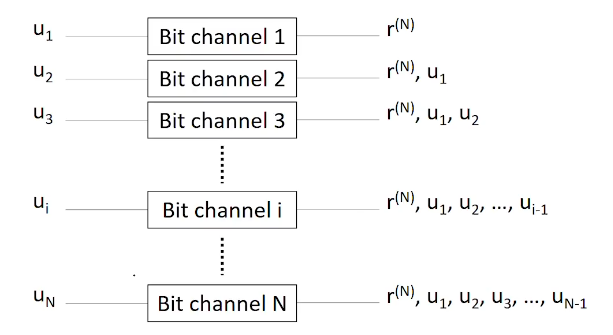
\includegraphics[width=0.5\textwidth, height=0.22\textheight]{bitchannels.png}
\caption{Transforming group of bits to each bit channel}
\end{figure}
The trick here is that, we will assume that the output vector $r^{(N)}$ does contain the information about the bit $u_{1}$. Similarly, for the $i^{th}$ bit channel also, we will assume that the outputs are $r^{(N)}, u_{1}, u_{2}, ..., u_{i-1}$. For now, let us assume that we are getting the previous bits at the output of a bit channel from somewhere. 
\par The properties of these bit channels is quite different. If we would have not applied the polar transform, the channel through which the bits would have gone would be same for all the bits. But now, each channel has a different property; why? Because the outputs of each bit channel is different. These properties are based upon the quality of the channels. The extremes of these bit channels are \textit{good} and \textit{bad}. There is nothing in between. That is why, this is called \textbf{channel polarization}.
\subsection{Reliability Sequence}
The reliability sequence is something that tells which bit channels are the good ones and which are the bad ones. For example, 1 2 3 5 4 6 7 8 is a reliability sequence. If we carefully look at it, we find that channel 5 is more bad as compared to channel 4. The current 5G standard uses 1024 length reliability sequence.
\section{The $(N, K)$ Polar Code}
The $(N, K)$ polar code is simple. Here we take $N = 2^{n}$ for some integer value of $n$. The value of $N>K$; this is a condition for the polar code. Now, we create a vector $U$ of length $N$, such that \begin{center} $U=\Big[u_{i}|i \in [1, N]\Big]$ \end{center}
\par Out of these $N$ input bits, we then set the first $(N-K)$ bits to 0, because, according to the reliability sequence, the initial bits are worst. The remaining $K$ bits in the reliability sequence are replaced by the message bits. So, the new $U$ vector is
\begin{equation}
U = \Big[ 0, 0, 0,...., 0_{(N-K)^{th}}, m_{1}, m_{2}, ...., m_{K} \Big]
\end{equation}
After this, we apply the polar transform on this $U$ vector to generate the codeword.
\begin{center}
$C=UG_{N}$
\end{center}
Where, $C$ is the codeword matrix and $m_{i}$ denotes the $i^{th}$ bit of the message. Let us illustrate this with the help of an example of $(8, 4)$ polar code. The reliability sequence is 1 2 3 5 4 6 7 8. We freeze the first $8-4=4$ bits by 0. The $U$ vector becomes $U=[0, 0, 0, m_{1}, 0, m_{2}, m_{3}, m_{4}]$. The codeword matrix is given by,
\begin{center}
$C = UG_{8}$
\end{center}
where, $G_{8}$ is
\[
G_{8} =
\begin{bmatrix}
1 & 0 & 0 & 0 & 0 & 0 & 0 & 0 \\
1 & 1 & 0 & 0 & 0 & 0 & 0 &0 \\
1 & 0 & 1 & 0 & 0 & 0 & 0 & 0 \\
1 & 1 & 1 & 1 & 0 & 0 & 0 & 0 \\
1 & 0 & 0 & 0 & 1 & 0 &0 &0 \\
1 & 1 & 0 & 0 & 1 & 1 & 0 &0 \\
1 & 0 & 1 & 0 & 1 & 0 &1& 0 \\
1 & 1 & 1 & 1 & 1 & 1 & 1 & 1 &\\
\end{bmatrix}
\]
Therefore, the $C$ matrix is 
\begin{center}
\[
C =
\begin{bmatrix}
\displaystyle \sum_{i=1}^{4}m_{i} \\
m_{1} + m_{2} + m_{4} \\
m_{1} + m_{3} + m_{4} \\
m_{1} + m_{4} \\
m_{2} + m_{3} + m_{4} \\
m_{2} + m_{4} \\
m_{3} + m_{4} \\
m_{4}
\end{bmatrix}
^{T}
\]
\end{center}
Where the additions correspond to the modulo 2 addition of the bits.
\section{Successive Cancellation}
In this part, we will see how to decode a given polar code. Although an intutive way could be to post multiply $G_{N}^{-1}$ to the codeword matrix, i.e.;
\begin{center}
$U = CG_{N}^{-1}$
\end{center} 
But this method is computationally costly. However, for the simulation purposes, we have taken this approach only, because it is easy to code and we just wanted to analyse polar codes as a whole.
\par We will now see a more better option to decode.
\par First, let us consider the extra outputs that we were getting in the bit channels apart from the $r^{(N)}$ vector. Consider bit channel 2; in this the output was the $r$ vector and the previous bit $u_{1}$. Now, if the bit $u_{1}$ was frozen, there is no need to do any calculation for the output bit of this kind. However, if it isn't, then the best we can do is, to estimate $u_{1}$ given the output vector $r$ and the nature of the bit channel 2 (see figure 5).
\begin{figure}[H]
\centering 
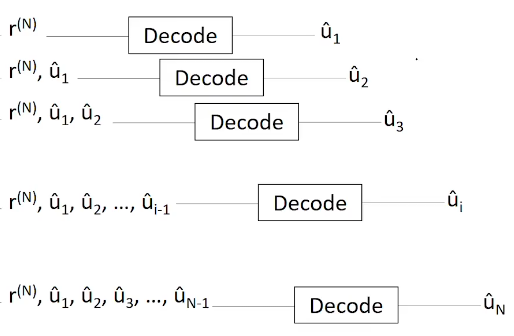
\includegraphics[width=0.5\textwidth, height=0.22\textheight]{decode.png}
\caption{Decoding the Polar Codes}
\end{figure}
The idea behind decoding such outputs is very simple. For the first bit channel, we pass the $r$ vector as it is to the decoder. According to figure 5, we will get an estimate of $u_{1}=\hat{u_{1}}$. We then pass the same vector $r$ to the next decoder alongwith $\hat{u_{1}}$ and decode $u_{2}$. Fortunately, by the very nature of the polar codes, the first $N-K$ bits will surely be zero, and therefore, there won't be much computations for the few initial decoders. 
\section{Results and Conclusions}
We now discuss the results and conclusions of our experimentation. When we started, we first compared the $BER$ vs $E_{b}/N_{o}$ ratio plot of uncoded and the coded case. We found the following results based on our simulation.
\begin{figure}[H]
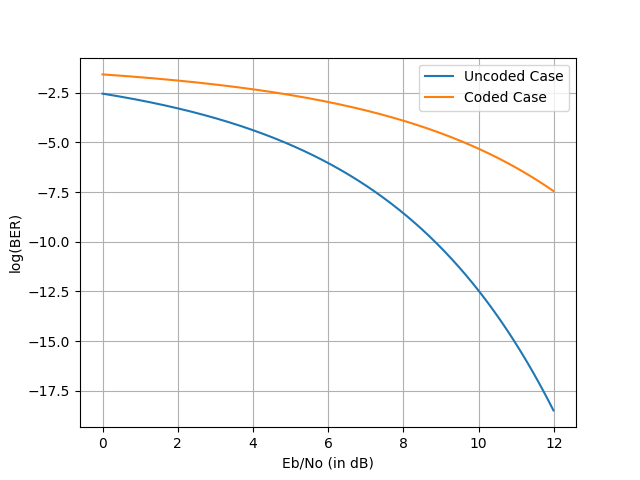
\includegraphics[width=0.5\textwidth, height=0.3\textheight]{codedvsuncoded.png}
\caption{$\log{BER}$ vs $E_{b}/N_{o}$ ratio for Uncoded and Coded case}
\end{figure}
Let us now understand why this happens. In the uncoded case $R=1$ and therefore, the bit error rate was $\displaystyle Q\Bigg(\sqrt{\frac{2E_{b}}{N_{o}}}\Bigg)$. But when the rate increased to some value $R$ such that $R \in (0,1)$ then the BER becomes $\displaystyle Q\Bigg(\sqrt{\frac{2RE_{b}}{N_{o}}}\Bigg)$. Clearly, 
\begin{center}
$\displaystyle Q\Bigg(\sqrt{\frac{2E_{b}}{N_{o}}}\Bigg) < \displaystyle Q\Bigg(\sqrt{\frac{2RE_{b}}{N_{o}}}\Bigg)$
\end{center}
for the same $E_{b}/N_{o}$ value. This is because $R<1$ and therefore, the argument of RHS $Q$ function is less than LHS $Q$ function, which implies the current relation. For more information, please refer section 1.6.
\par Later on, we also saw the $(7, 4)$ Hamming code. The below shown graph shows that for higher values of $E_{b}/N_{o}$, the method of decision does not matter much. We can either use soft decision or hard decision.

\begin{figure}[H]
\centering 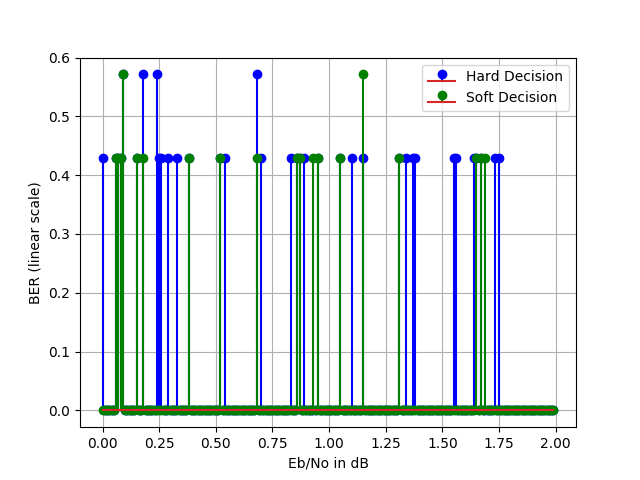
\includegraphics[width=0.6\textwidth, height=0.25\textheight]{hamming.png}
\caption{Soft decision vs. Hard decision}
\end{figure}
This graph is also the result of the simulation.
\par We now come to main simulation concerning the polar codes. We conducted two types of simulations here. In the first type of the simulation, we varied the message length (in bits) from 1 to 16 and for each length we calculated the average BER with $E_{b}/N_{o}$ ratio varying from 0 to 12 in the steps of 0.01. On the successful simulation we found that for small message lengths the average BER is more than those with higher message lengths. The graph shown below, conveys the same thing.
\begin{figure}[H]
\centering 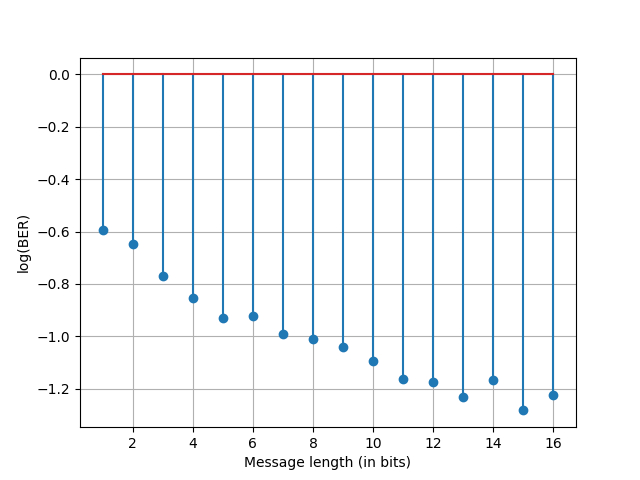
\includegraphics[width=0.6\textwidth, height=0.25\textheight]{polar1.png}
\caption{Average BER for differnt message bit length}
\end{figure}
This is happening because the logarithm is getting more and more negative. Therefore, based on our simulation, \textbf{we conclude that polar codes are good when $K \rightarrow N$}.

\par The second type of test that we conducted was by fixing the message length and varying the $E_{b}/N_{o}$ ratio, just like we did with Hamming code and repitition code. The graph for this test is shown below.
\begin{figure}[H]
\centering 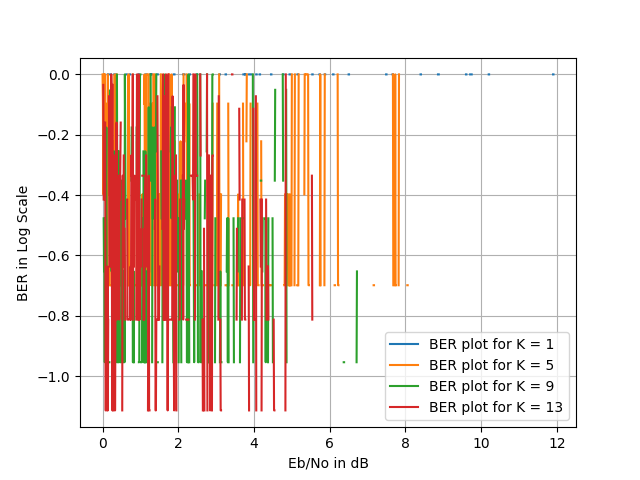
\includegraphics[width=0.55\textwidth, height=0.4\textheight]{polar2.png}
\caption{Average BER for differnt message bit length}
\end{figure}
Since this plot is also in the logarithmic scale, we need to be little cautious while reading it. The peaks having less height are more worse than those having high peaks. This is because the logarithm is negative, which means that the higher the negative log, the lesser is the linear scale value. Again, this graph shows the same results as were shown by figure 8 above. For larger message lengths, the polar code is favourable. Note that the tests conducted here were based on $(16, K)$ type polar codes where $K\leq16$.
\par Apart from these simulations also, polar codes have various advantages. The most obvious one is the time complexity which is $\mathcal{O}(n\log{n})$. On the other hand, repitition codes have poor error correcting capabilities. Polar codes have helped achieve high throughput in 5G wireless network when used as channel coding. During 5G field trials, Huawei has achieved 27 Gbps. 

\section{References}

[1] Polar Codes: Primary Concepts and
Practical Decoding Algorithms, Kai Niu, Kai Chen, Jiaru Lin, and Q. T. Zhang 0163-6804/14/\$25.00 © 2014 IEEE \\

[2] https://nptel.ac.in/courses/108106137/26 \\

[3] https://dsp.stackexchange.com
\end{document}